\documentclass{article}
\usepackage[utf8]{inputenc}

\usepackage{amssymb,amsmath}
\usepackage{mathrsfs}

\usepackage{hyperref}
\usepackage{graphicx}

\usepackage[top=3cm, bottom=3cm, left=3cm, right=3cm, includefoot]{geometry}

%\usepackage{multirow} % multirow in tables
%\usepackage{hhline} 
\usepackage{xcolor,colortbl}
\usepackage{array}
%\newcolumntype{L}[1]{>{\raggedright\let\newline\\\arraybackslash\hspace{0pt}}m{#1}}
%\newcolumntype{C}[1]{>{\centering\let\newline\\\arraybackslash\hspace{0pt}}m{#1}}
%\newcolumntype{R}[1]{>{\raggedleft\let\newline\\\arraybackslash\hspace{0pt}}m{#1}}

\usepackage{arydshln} % dash lines in arrays (for separation of matrix elements)


\DeclareMathOperator{\tr}{\mathrm{trace} }

\newcommand{\MakeTitlePage}
{
  \begin{center}
    \vspace{10mm}
    \sffamily
    {\huge\bfseries
    {HPC-Causality report}\\
    }
    \bigskip
    \bigskip
    {\large
	 \vspace{0.5cm}
	 {Illia Horenko, Patrick Gagliardini, William Sawyer, \underline{Luk\'{a}\v{s} Posp\'{i}\v{s}il}}	
    }
  \end{center}
  \vspace{10mm}
  \hrule
}

\newcommand{\todo}[1]{{\color{red}TODO: #1}} % todo command
\renewcommand\contentsname{\sffamily{}} % no title of content

\begin{document}
 \MakeTitlePage
 \tableofcontents
 \newpage

 \section {The problem}

 In our project, we analyze the time-series, i.e. the sequence of given data
 \begin{equation}
  \label{eq:timeseries}
	x_0, x_1, \dots, x_{T-1},
 \end{equation}
 where $x_t \in \mathbb{R}^{\mathrm{xdim}}$ and $\mathrm{xdim} \in \mathbb{N}$ is the number of values (measurements) in each time step. 
 We try to understand the inner mechanism (dynamics) of the sequence. \newline
 
 As the first step of analyze of given data, we can use classical tools and easily compute "static"\footnote{I decided to use this term, because following properties does not take into account the time} statistics, like average, variance, deviation and other moments or central moments.
 These values provide us the basic properties of the given set of data, however they does not take into account the fact, that we are not working with only set, but we analyze the sequence.

 One of the most typical way how to analyze sequences is to appoximate the given data by much more simplier function. Afterwards, analyzing this approximating function provides us the basic knowledge of sequence behaviour with respect to time. 
 The approximation is performed to be "as good as possible", i.e. in a such way, that the error of the approximation is as small as possible.
 
 The most simplest approximation function is linear\footnote{in fact, the simplest approximation function is constant function; however the constant function is in this case the average of given set of data; constant function is constant with respect to time and therefore it cannot reflect the dynamics of the sequence}.
 In this case, we are talking about \emph{linear regression}.
 
 For the simplicity, in the following we will suppose one dimensional data $\mathrm{xmem} = 1$, i.e. $x(t) \in \mathbb{R}$. 
 Provided observations could be easily generalized to more dimensions.
 
 Suppose that all given data \eqref{eq:timeseries} linearly depends on the time, i.e. each data point could be written in form $x(t) = \alpha_0 + \alpha_1 t$, where $\alpha_0,\alpha_1 \in \mathbb{R}$ are unknown time-independent parameters of this linear \emph{model}. 
 However, general sequence is not generated by linear function, therefore in each time-step we make an error. To be more exact, we rather write
 \begin{equation}
  \label{eq:linear}
  x(t) = \alpha_0 + \alpha_1 t + \varepsilon_t, ~~t = 0,\dots,T,
 \end{equation}
 where $\varepsilon_t$ is an error of approximation (hopefully small for all $t$). 
 If we denote 
 \begin{displaymath}
  \begin{array}{rcl}
   x & = & [x_0, \dots, x_{T-1}]^T \in \mathbb{R}^T, \\[5mm]
   Z & = & \left[
    \begin{array}{ccccc}
     1 & 1 & 1 & \dots & 1 \\
     0 & 1 & 2 & \dots & T-1
    \end{array} 
     \right] \in \mathbb{R}^{2,T}, \\[5mm]
   y & = & [\alpha_0,\alpha_1]^T \in \mathbb{R}^2, \\[5mm]
   \varepsilon & = & [\varepsilon_0,\dots,\varepsilon_{T-1}] \in \mathbb{R}^T,
  \end{array}
 \end{displaymath}
 then the system of equations \eqref{eq:linear} could be written in form
 \begin{equation}
  \label{eq:linear2}
  x = Z^T y + \epsilon.
 \end{equation}
 We want to perform the approximation (i.e. find $y$) in the best way as possible. We minimize the size of the error $\Vert \varepsilon \Vert \rightarrow \min\limits_{y}$. 
 Using \eqref{eq:linear2}, we can substitute and we get optimization problem
 \begin{equation}
  \label{eq:linear_opt}
  \hat{y} = \arg\min\limits_{y} \Vert \varepsilon \Vert  = \arg\min\limits_{y} \Vert Z^T y - x \Vert = \arg\min\limits_{y} \underbrace{\frac{1}{2}\Vert Z^T y - x \Vert^2}_{ = \Psi(y)}  
 \end{equation}
 Please, notice that $\Psi(y)$ is quadratic function
 \begin{displaymath}
  \Psi(y) = \frac{1}{2}\Vert Z^T y - x \Vert^2 = \frac{1}{2}\langle Z^T y - x, Z^T y - x \rangle = \frac{1}{2}y^T Z Z^T y - y^T Z x + \frac{1}{2}x^T x,
 \end{displaymath}
 therefore the gradient is given by
 \begin{displaymath}
  \nabla \Psi(y) = ZZ^T y - Z x
 \end{displaymath}
 and the necessary optimality condition of \eqref{eq:linear_opt} is given by the system of linear equations\footnote{yes, this is a least-square solution of our first naiive approach $x(t) = \alpha_0 + \alpha_1 t$}
 \begin{displaymath}
  ZZ^T y = Zx .
 \end{displaymath}

% \begin{example}
%  Let us consider data
%  \begin{displaymath}
%   x_0 = 
%  \end{displaymath}
% \end{example}

 Using a simple generalization idea, we are able to extend the linear regression model to polynomial models
 \begin{displaymath}
  x(t) = p(t) + \varepsilon_t, p \in \mathcal{P}_n,
 \end{displaymath}
 where $\mathcal{P}_n$ is a vector space of polynomial function of degree $n \in \mathbb{N}$.
 
 \section {VarX model}

 In this model, we suppose that the data was generated using linear recursive formula
 \begin{equation}
  \label{eq:varx_stationary}
	x_t = \mu + \sum\limits_{q=1}^{\mathrm{xmem}} A_q x_{t-q} + \sum\limits_{p=0}^{\mathrm{umem}} B_p u_{t-p} + \varepsilon_t, \forall t = \mathrm{xmem}, \mathrm{xmem}+1, \dots, T-1,
 \end{equation}
 where given data $x_t \in \mathbb{R}^{\mathrm{xdim}}, t = 0,\dots,T-1$ are stored in column vectors, $A_q \in \mathbb{R}^{\mathrm{xdim},\mathrm{xdim}}$ are unknown coefficients (matrices) corresponding to previous $\mathrm{xmem}$ time-steps and \todo{write here something funny about variables in the model}.
  
 Let us denote the number of equations in \eqref{eq:varx_stationary} by $m = T-\mathrm{xmem}$.
 Moreover, we define 
 \begin{displaymath}
  \begin{array}{rcl}
   X & = & [x_{\mathrm{xmem}}, x_{\mathrm{xmem}+1}, \dots, x_{T-1}] \in \mathbb{R}^{\mathrm{xdim},m} \\[5mm]
   M & = & [\mu, A_1, A_2, \dots, A_{\mathrm{xmem}}, B_0, B_1, \dots, B_{\mathrm{umem}} ] \in \mathbb{R}^{\mathrm{xdim},1+\mathrm{xmem}\cdot\mathrm{xdim}+(\mathrm{umem}+1)\cdot\mathrm{udim}}\\[5mm]
   Z & = & \left[
	\begin{array}{ccccc}
	 1 & 1 & 1 & & 1 \\ \hdashline[2pt/2pt]
	 x_{\mathrm{xmem}-1} & x_{\mathrm{xmem}} & x_{\mathrm{xmem}+1} & & x_{T-1} \\
	 \vdots & \vdots & \vdots & \dots & \vdots \\
	 x_0 & x_1 & x_2 & & x_{T-\mathrm{xmem}} \\ \hdashline[2pt/2pt]
	 u_{\mathrm{xmem}} & u_{\mathrm{xmem}+1} & u_{\mathrm{xmem}+2} & & u_{T-1} \\
	 u_{\mathrm{xmem}-1} & u_{\mathrm{xmem}} & u_{\mathrm{xmem}+1} & & u_{T-2} \\
	 \vdots & \vdots & \vdots & & \vdots 
    \end{array}
   \right] \in \mathbb{R}^{1+\mathrm{xmem}\cdot\mathrm{xdim}+(\mathrm{umem}+1)\cdot\mathrm{udim},m} \\[5mm]
   \varepsilon & = & [\varepsilon_{\mathrm{xmem}}, \varepsilon_{\mathrm{xmem}+1}, \dots, \varepsilon_{T-1}] \in \mathbb{R}^{\mathrm{xdim},m}
  \end{array}
 \end{displaymath}

 Then \eqref{eq:varx_stationary} is equivalent to\footnote{please, notice that both of left side and right side are matrices}
 \begin{equation}
  \label{eq:varx_stationary_matrix}
  X = MZ + \varepsilon,
 \end{equation}
 where $M$ is matrix of unknown parameters of the model \eqref{eq:varx_stationary}.
 Now we will find $M$ as \emph{the best} solution, i.e. we minimize the size of error $\varepsilon$ in \eqref{eq:varx_stationary_matrix}\footnote{please, notice that we are talking about matrix norms}
 \begin{displaymath}
  \label{eq:eq:varx_stationary_matrix_eps}
  \Vert \varepsilon \Vert = \Vert X - MZ \Vert ~~ \rightarrow ~~ \min\limits_{M}.
 \end{displaymath}
 or equivalently\footnote{\todo{the trace and matrix norms should be discussed}}
 \begin{displaymath}
   \bar{M} =  \arg \min\limits_{M} \Vert X - MZ \Vert =  \arg \Vert X - MZ \Vert^2 =  \arg \min\limits_{M} \underbrace{\tr\Vert X - MZ \Vert^2}_{= L(M)}.
 \end{displaymath}
 The optimization problem with object function $L(M): \mathbb{R}^{\mathrm{xdim},1+\mathrm{xmem}\cdot\mathrm{xdim}+(\mathrm{umem}+1)\cdot\mathrm{udim}} \rightarrow \mathbb{R}^{+}_0$ could be simplified 
 \begin{displaymath}
  \begin{array}{rcl}
   \min L(M) & = & \min \tr \Vert X - MZ \Vert^2 = \min \tr (X-MZ)^T(X-MZ) \\
        & = & \min \tr \left( X^TX - X^TMZ - (MZ)^TX + (MZ)^T MZ \right) \\
        & = & \min \tr \left( X^TX - X^TMZ - Z^TM^TX + Z^T M^T MZ \right) \\
        & = & \min \tr (X^TX) - \tr (X^TMZ) - \tr (Z^TM^TX) + \tr (Z^T M^T MZ)
  \end{array}
 \end{displaymath}
 We consider the neccessary optimality condition $\frac{\partial L(M)}{\partial M} = 0$, therefore we have to compute the derivatives of addends in the previous formula.
 These derivatives follow (using \cite{matrix_cookbook}\todo{add cookbook reference}).
 \begin{displaymath}
  \begin{array}{rcl}
   \frac{\partial \tr (X^TX)}{\partial M} & = & 0 \\
   \frac{\partial \tr (X^TMZ)}{\partial M} & = & XZ^T \\
   \frac{\partial \tr (Z^TM^TX)}{\partial M} & = & XZ^T \\
   \frac{\partial \tr (Z^TM^T M Z)}{\partial M} & = & M(ZZ^T) + M (ZZ^T) = 2MZZ^T
  \end{array}
 \end{displaymath}
 Therefore the neccessary optimality condition of the problem \eqref{eq:eq:varx_stationary_matrix_eps} is given by
 \begin{displaymath}
  \frac{\partial L(M)}{\partial M} = 0 ~~~ \Leftrightarrow ~~~ -2XZ^T + 2M(ZZ^T) = 0,
 \end{displaymath}
 which could be written in the form of the system of linear equations with multiple right-hand side vectors as
 \begin{equation}
  \label{eq:varx_stationary_system}
  (ZZ^T) M^T = ZX^T,
 \end{equation}
 where $M^T$ is the matrix of unknown parameters of the original model \eqref{eq:varx_stationary}.

 \subsection{Checking equations by example}
 
 Let us consider a problem with $\mathrm{xdim} = 2, \mathrm{udim} = 1, \mathrm{xmem} = 2, \mathrm{umem} = 0, T = 5$. Then $m = 3$ and
 \begin{displaymath}
  X \in \mathbb{R}^{2,3}, ~ M \in \mathbb{R}^{2,6}, ~ Z \in \mathbb{R}^{6,3}, ~\varepsilon \in \mathbb{R}^{2,3}.
 \end{displaymath}
 Please, see Fig. \ref{fig:varx1}, where we present given data (time-series and external forces) and Fig. \ref{fig:varx2} to visualize objects in the problem.
 
 \begin{figure}[h!]
  \centering
    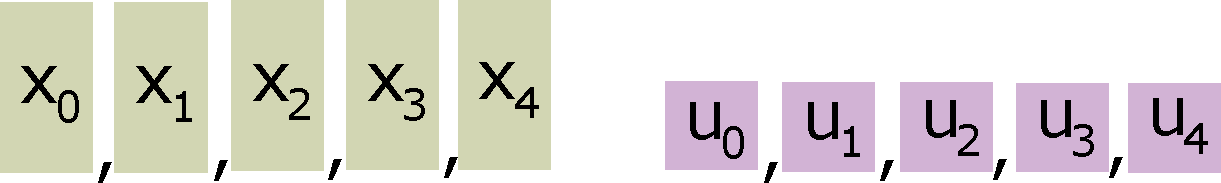
\includegraphics[scale=0.2]{varx1.pdf}
  \caption{Given data in VarX problem; time-series values $x_0,x_1,x_2,x_3,x_4$ and external forces $u_0,u_1,u_2,u_3,u_4$.}
  \label{fig:varx1}
 \end{figure}

 \begin{figure}[h!]
  \centering
    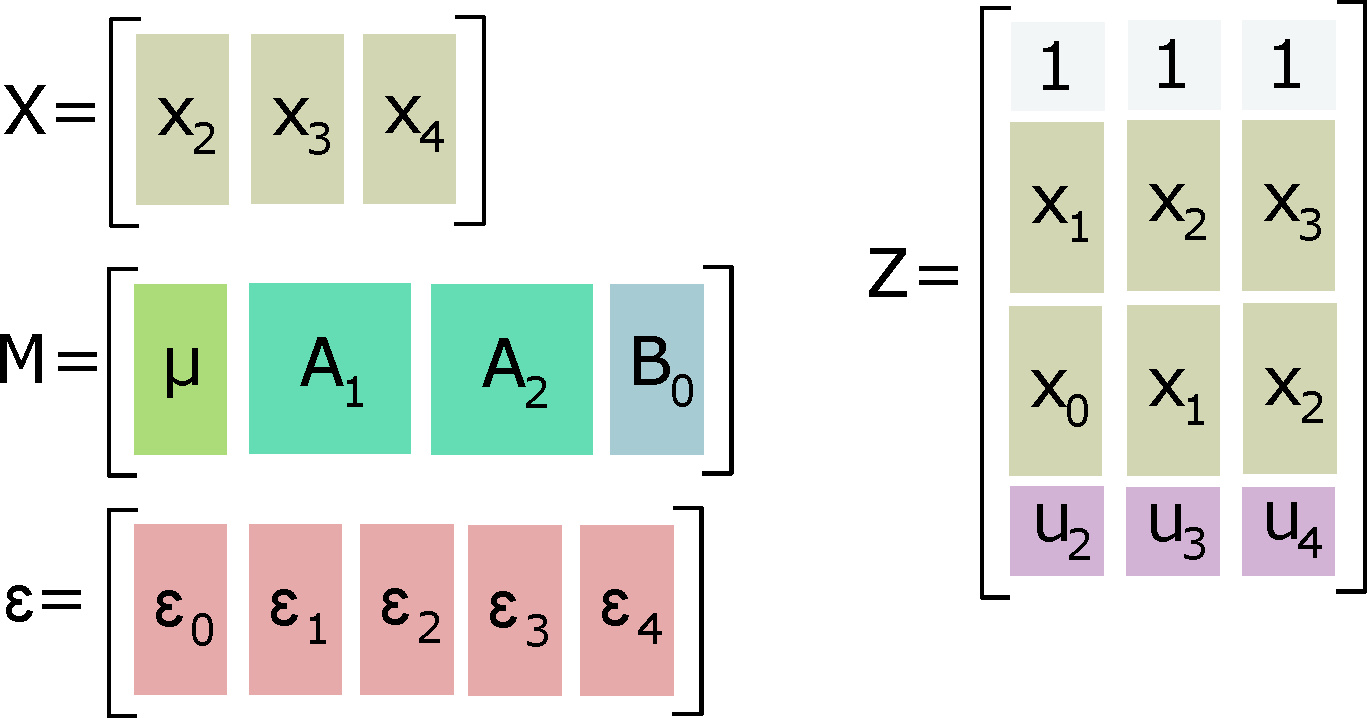
\includegraphics[scale=0.2]{varx2.pdf}
  \caption{Objects in the VarX problem.}
  \label{fig:varx2}
 \end{figure}

 The most complicated operation in equation \eqref{eq:varx_stationary_matrix} is matrix multiplication $MZ$. The graphical analysis of this operation could be found in Fig. \ref{fig:varx3}.
 Here, we used general property
 \begin{displaymath}
  \forall A \in \mathbb{R}^{m,n} \forall v_1,v_2 \in \mathbb{R}^n: A\left[ v_1, v_2 \right ] = \left[ A v_1, Av_2 \right] ,
 \end{displaymath}
 i.e. multiplication by matrix could be applied into columns.

 \begin{figure}[h!]
  \centering
    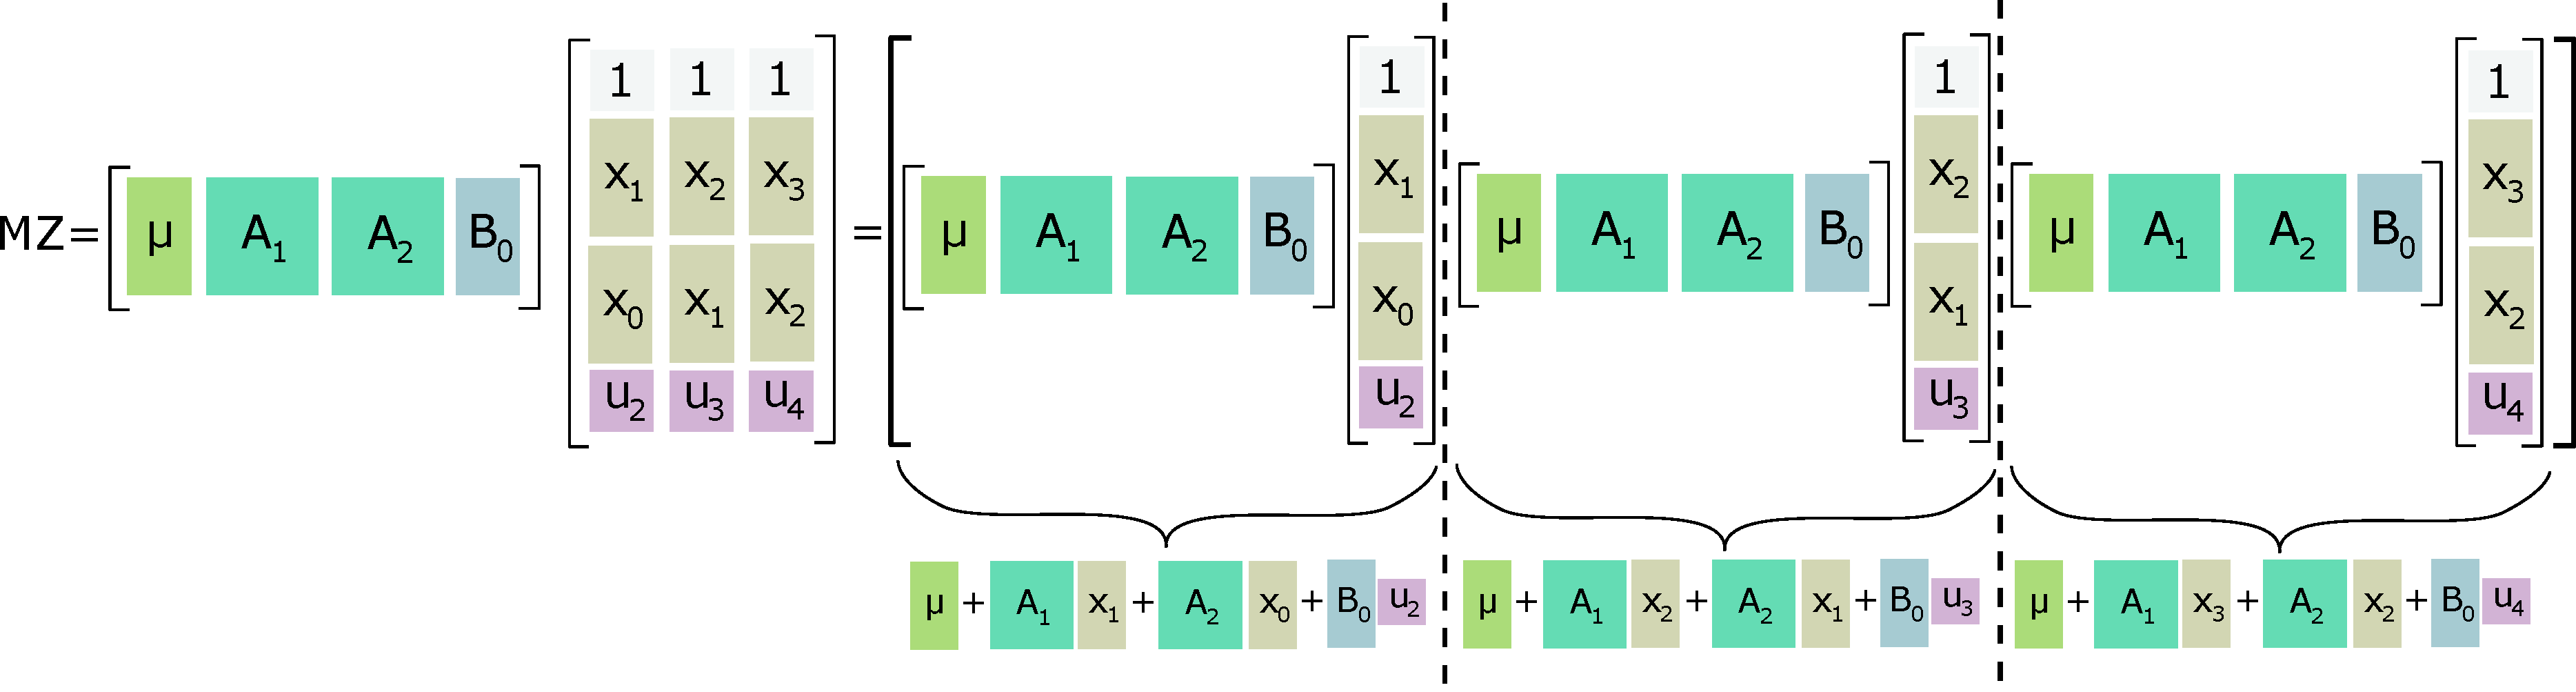
\includegraphics[scale=0.2]{varx3.pdf}
  \caption{Multiplication $MZ$; the dashed line represents the separation between columns.}
  \label{fig:varx3}
 \end{figure}
 
 Now we are ready to assemble $X = MZ + \varepsilon$ (which we actually will not demonstrate, because the operation addition on the right side is an operation between columns of matrices, it is trivial, and it will be clear from following).
 Afterwards, we can compare columns on the left and right side of equation $X = MZ + \varepsilon$, see Fig. \ref{fig:varx4} and we obtain the original equations in VarX model, see equations \eqref{eq:varx_stationary}.
 Therefore, in this case, equations \eqref{eq:varx_stationary} and \eqref{eq:varx_stationary_matrix} are equivalent.

 \begin{figure}[h!]
  \centering
    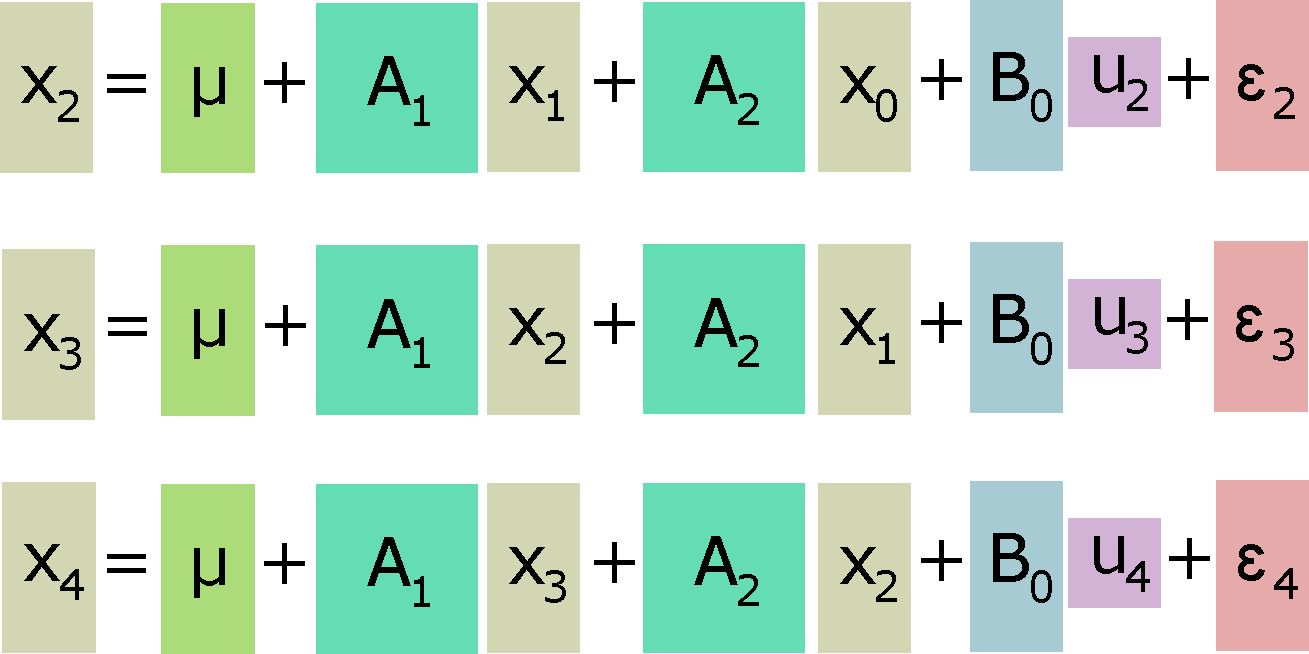
\includegraphics[scale=0.2]{varx4.pdf}
  \caption{The definition of original VarX problem.}
  \label{fig:varx4}
 \end{figure}

 \section {Non-stationary VarX model}

 Let us consider a VarX model \eqref{eq:varx_stationary}, where the coefficients depend on the time (vary during time)
 \begin{equation}
  \label{eq:varx_nonstationary}
	x_t = \mu(t) + \sum\limits_{q=1}^{\mathrm{xmem}} A_q(t) x_{t-q} + \sum\limits_{p=0}^{\mathrm{umem}} B_p(t) u_{t-p} + \varepsilon_t, \forall t = \mathrm{xmem}, \dots, T-1
 \end{equation}
 In this case, we are talking about non-stationary VarX model. Please notice, that the problem is ill-posted, theoretically each $x_t$ could have its own parameters $\mu,A,B$ and
 obtained results could be biased and consequently useless. Therefore, we rather split the time $t=\mathrm{xmem},\dots,T-1$ into finite number of clusters (denoted by $K \geq 1$)
 and we will suppose that the part of time-series corresponding to each cluster could be described by one specific stationary VarX model (model with constant, i.e. time-independent, parameters $\mu^k,A^k,B^k, k = 0,\dots,K-1$ in corresponding part of time-series). \newline
 
 The switching between $K$ models is realized by model indicator functions\footnote{please, see (i.e. google) the formal mathematical definition of \emph{indicator function} of general set; I decided to use this terminology, because in the case of modelling, it describes the same indicator property}
 $\gamma_k(t), k=0,\dots,K-1, t = \mathrm{xmem},\dots,T-1$ defined by
 \begin{equation}
  \label{eq:gamma}
  \gamma^k(t) =
  \left\lbrace
   \begin{array}{ll}
    1 ~~~ & \textrm{if $k$-th cluster-model is active in time $t$,} \\
    0 ~~~ & \textrm{if $k$-th cluster-model is not active in time $t$.}
   \end{array}
  \right.
 \end{equation} 

 Moreover, we demand that there is only one cluster-model active in each time step $t$. This property could be described by condition
 \begin{equation}
  \label{eq:gamma_eq}
  \forall t = \mathrm{xmem}, \dots, T-1: ~~ \sum\limits_{k=0}^{K-1} \gamma^k (t) = 1,
 \end{equation}
 i.e. the sum of indicators functions $\gamma^k$ in each time-step is equal to one. Since these indicator functions are defined by \eqref{eq:gamma}
 as a functions, which attain $0$ or $1$, the equality condition \eqref{eq:gamma_eq} could be interpreted as follows: there is exactly one cluster-model
 active in each time-step.
 
 Using clustering and indicator functions, the non-stationary VarX model \eqref{eq:varx_nonstationary} could be written in form (we denote $\gamma^k(t) = \gamma^k_t$)
 \begin{equation}
  \label{eq:varx_nonstationary_gamma}
   \
	x_t = 
	\sum\limits_{k=0}^{K-1} 
	\sum\limits_{t=\mathrm{xmem}}^{T-1} 
	\left[
	 \gamma^k_t
	 \left( \mu^k + \sum\limits_{q=1}^{\mathrm{xmem}} A_q^k x_{t-q} + \sum\limits_{p=0}^{\mathrm{umem}} B_p^k u_{t-p} \right)
	\right] 
	+ \varepsilon_t, \forall t = \mathrm{xmem}, \dots, T-1.
 \end{equation}
 Please, notice that now the problem is much more complicated; we have to find not only the parameters $\mu^k, A^k,B^k$ of each cluster-model, but also the values of characteristic functions $\gamma^k$.

 Using the similar notations as in stationary case, we are able to define the optimization problem (the problem for minimization of the size of the modelling error, i.e. fitting error) as\footnote{\todo{discuss more deeply}} 
 \begin{displaymath}
  \label{eq:eq:varx_nonstationary_matrix_eps}
  \sum\limits_{k=0}^{K-1} \Vert X - M^k Z \Vert^2 ~~ \rightarrow ~~ \min\limits_{M^0,\dots,M^{K-1}, \gamma^{0}, \dots, \gamma^{K-1}}.
 \end{displaymath} 
 Here we denoted $\gamma^k = [\gamma^k_{\mathrm{xmem}}, \dots, \gamma^k_{T-1} ]^T \in \mathbb{R}^m$.
 
 \section {K-means model as a patological case of non-stationary VarX model}

 Let us consider a VarX model \eqref{eq:varx_stationary} with $\mathrm{xmem} = 0$ and without external forces term $u_t$
 \begin{equation}
  \label{eq:kmeans_stationary}
  x_t = \mu + \varepsilon_t, \forall t = 0,\dots,T-1.
 \end{equation}
 Please notice, that in this case we are trying to approximate whole time-series by a single value. It is not surprise, that this value is the average value of all $x_t$;
 see the solution of system \eqref{eq:varx_stationary_system}. In this case $Z = [1,\dots,1] \in \mathbb{R}^n$, the matrix $ZZ^T = T$, and the solution is given by
 \begin{displaymath}
  M^T = \mu^T = \frac{1}{T} \sum\limits_{t=0}^{T-1} x_t^T.
 \end{displaymath}
 Much more interesting is the non-stationary version of the model \eqref{eq:kmeans_stationary}. In this case, we are going to cluster the time-series into the set of clusters,
 where each cluster is characterized by one mean value. This model is well-known as \emph{K-means}.

\end{document} 
 
